\vspace{1cm}

\textbf{Àlex Giménez-Romero$^{1}$, Maialen Iturbide$^{2}$, Eduardo
    Moralejo$^{3}$, Jose M. Gutiérrez$^{2}$, Manuel A. Matías$^{1}$}

\vspace{1cm}

\begin{enumerate}
    \small
    \item Instituto de Física Interdisciplinar y Sistemas Complejos, IFISC
          (CSIC-UIB), Palma de Mallorca 07122, Spain
    \item Instituto de Física de Cantábria (CSIC-University of Cantabria),
          Avenida de los Castros, 39005 Santander, Spain
    \item Tragsa, Passatge Cala Figuera 6, 07009 Palma de Mallorca, Spain
\end{enumerate}

\vspace{1cm}

\textbf{Published as}

\vspace{0.5cm}

\fullcite{GimenezRomero2023_PD}

\newpage
\section{Introduction}

Climate change is widely recognized as an important driver of shifts in the
distribution and prevalence of plant diseases worldwide
\cite{harvell2002climate, Delgado-Baquerizo2020,  Rocklov2020, Dudney2021,
    Chaloner2021, Singh2023}. Although the impact of climate change on the
distribution of plant diseases has been approached from various perspectives
\cite{bergot2004simulation,pangga2011pathogen}, few studies have considered
epidemiological dynamics in climate projections
\cite{bebber2019climate,Juroszek2015}. Modeling disease epidemics is a complex
task, as they are emergent phenomena resulting from non-linear interactions
between disease components. In addition, many of the processes involved in
disease development also exhibit non-linear responses to changes in
environmental variables \cite{scherm1994global,garrett2011complexity}. This
complexity is further exacerbated in the case of vector-borne plant diseases
\cite{jeger2019epidemiology}. While climate primarily determines the potential
geographic range of each organism in the pathosystem, the development of
epidemic outbreaks depends on favorable host-pathogen-vector-climate
interactions that drive transmission chains. Consequently, modeling the risk of
vector-borne plant diseases implies delimiting their epidemiological niche
rather than the ecological niche of their parts, as is commonly done.

The emergence of \textit{X. fastidiosa} in Europe has renewed interest in
modeling vector-borne plant diseases, particularly the risk they pose to the
European wine industry. Pierce's disease (PD) is an endemic fatal disease of
grapevines
in the Americas transmitted unspecifically by sap-feeding insect vectors
belonging to sharpshooter leafhoppers (Hemiptera: Cicadellinae) and spittlebugs
(Hemiptera: superfamily Cercopidae) \cite{redak2004biology}. In the US, PD
causes huge economic losses to the wine sector estimated at 100 M\$ per year in
California alone \cite{tumber2014pierce}. The causative agent of PD is
\textit{Xylella fastidiosa} (Xf), a bacterium capable of colonizing the xylem
vessels of more than 600 hosts, including important crops
\cite{delbianco2019new}. As a taxonomic unit, Xf comprises three recognized
subspecies, \textit{fastidiosa}, \textit{multiplex}, and \textit{pauca}, and
more than 90 sequence types (i.e. genetic lineages) with distinct host ranges.
Specifically, the Xf clonal lineage that causes Pierce's disease (hereafter
\xf) also causes almond leaf scorch in California \cite{almeida2003biological}.

Until the beginning of the 21st century, Xf was a pathogen officially
restricted to the American continent \cite{almeida2015plant}. In 2013, the
involvement of Xf subsp. \textit{pauca} in the massive death of ancient olive
trees in Apulia, Italy, and its rapid spread raised alarm in European
agriculture \cite{saponari2013identification}. Today, all three Xf subspecies
have been detected in the Balearic Islands (Spain), including \xf{}, and
several clonal lineages have been found in Corsica and the PACA region of
France, Alicante (Spain), Tuscany (Italy) and Portugal
\cite{olmo2021landscape,denance2017several,marco2021evidence}. Outside North
America, \xf{} is only established on the islands of Mallorca and Taiwan, and
has recently been detected in Israel, Lebanon and Portugal
\cite{zecharia2022xylella,carvalho2022dispersion}. In all European outbreaks,
the insect vector \textit{Philaenus spumarius} is the main and almost unique
carrier of Xf \cite{cornara2018philaenus}.

Despite recent studies agree that the current risk of PD establishment in
Europe is primarily confined to the Mediterranean basin
\cite{godefroid2019xylella,Godefroid2022_vector,GimenezRomero2022_CommsBio},
its
potential future progression is not yet clear. Some efforts have been made to
characterize the geographical distribution of Xf-induced diseases in Europe
under climate change, but these are limited to the use of species distribution
models (SDMs) for the pathogen \cite{Bosso2016b,Schneider2020,Godefroid2022}
and the vector \cite{Godefroid2022_vector}, which have led to conflicting
results. On the one hand, higher temperatures are expected to promote bacterial
growth in susceptible crops in continental southern Europe, while on the other
hand, these areas are progressively experiencing drier environmental conditions
detrimental to vector populations \cite{Godefroid2022_vector}. Furthermore, the
use of SDMs to predict the potential distribution of vector-borne plant
diseases, while capable of providing good approximations, is generally
inadequate. The observed distribution of the pathogen cannot be separated from
that of the vector, especially in the case of obligate pathogens such as Xf.
Furthermore, the potential distribution of the pathogen or the vector alone
have no epidemiological meaning, what implies that they do not provide
quantitative predictions of the severity of the disease. In addition, a larger
set of available climate models is desirable to properly deal with the inherent
uncertainty in the predictions,

To overcome these limitations, here we use a novel climate-driven
epidemiological model of PD epidemic risk \cite{GimenezRomero2022_CommsBio}.
The model
determines the spatio-temporal epidemic risk based on the spatial distribution
of vectors, temperature-dependent bacterial growth and survival within hosts,
and subsequent epidemiological dynamics. The model forces the introduction of
the pathogen and examines whether the disease can establish and spread from
previous states under climatic conditions of the location. In
\cite{GimenezRomero2022_CommsBio} the model was used to determine the risk of
PD under
current climatic conditions in wine-growing regions worldwide, while a linear
regression was used to obtain a crude first estimate of the risk in the future.
This simple estimation is not expected to be reliable, because it overlooks the
role of nonlinearities in the model and also does not take into account climate
change scenarios (as described in the manuscript). To assess the potential
distribution and relative impact of PD on European vineyards under different
levels of global warming, here we used state-of-the-art regional climate
projections from the EURO-CORDEX initiative \cite{jacob_regional_2020}. Our
study takes into account uncertainties in climate projections and provides an
updated and comprehensive assessment of PD risk in European wine-growing
regions, addressing previous limitations. We posit that pest risk maps
constructed from projections of epidemiological models driven by climate data
provide a more realistic, quantitative and explanatory predictions than
correlative and probabilistic models. Additionally, they offer valuable
insights for anticipating and managing the potential impacts of PD and thus
ensuring the resilience of viticulture despite future climate challenges.

\section{Methods}\label{methods}

\subsection{Climate datasets}

We used E-OBS version v21e \cite{cornes_ensemble_2018} as the reference
observational climatic dataset, providing daily gridded data for Europe at a
resolution of 0.1 degrees ($\sim$10 km). Maximum and minimum temperature data
was used to compute the MGDD and CDD indices involved in the growth and
survival processes of the \xf{} pathogen (see ``Climate-driven epidemiological
model" section below). To calibrate the distribution models of \textit{P.
    spumarius} capturing the widest possible range (North America and Europe),
we
used the ERA5-Land reanalysis
\cite{munoz-sabater_era5-land_2021} due to its global (land) coverage and
high resolution (0.1 degrees, as E-OBS). Daily precipitation and daily minimum
and maximum temperature data were retrieved to calculate the moisture index and
maximum temperature during spring index required for the vector suitability
model (see ``Vector suitability" section below).
Historical and future projections of both indexes were calculated using
regional climate simulations from the state-of-the-art large high-resolution
(0.11 degrees) ensemble provided by EURO-CORDEX \cite{giorgi_regional_2015}.
This dataset includes daily simulations of precipitation and temperatures from
a large ensemble of Regional Climate Models (RCMs) driven by Global Climate
Models (GCMs) from the CMIP5 project \cite{Taylor_2011}. For this, we
considered the RCP8.5 simulations for 40 combinations of GCMs-RCMs
(\cref{tab:GCM-RCM}). In order to calculate 20-year mean climatic indexes
across the different global warming levels (+1.5ºC, +2ºC, +3ºC and +4ºC), we
relied on the time periods during which each CMIP5 driving model reaches the
designated level within the RCP8.5 scenario (see
\cite{diez-sierra_consistency_2023}). This information is available at the IPCC
WGI Atlas GitHub repository \cite{iturbide_repository_2021}.

\begin{table}[H]
    \centering
    \caption{\textbf{EURO-CORDEX GCM-RCM combinations used in this study.
            Numbers indicate the number of runs in each combination.}}
    \label{tab:GCM-RCM}
    \resizebox{\textwidth}{!}{%
        \begin{tabular}{l|l|l|l|l|l|l}
                                             & CNRM-CM5     & EC-EARTH   &
            HadGEM2-ES
                                             & IPSL-CM5A-MR & MPI-ESM-LR &
            NorESM1-M
            \\
            \hline
            CLMcom-CCLM4-8-17\_v1            & 1            & 1          & 1
                                             &              & 1          &
            \\
            \hline
            DMI-HIRHAM5\_v2                  & 1            & 1          & 1
                                             &              &            &
            \\
            \hline
            GERICS-REMO2015\_v2              & 1            &            &
                                             &              &            &
            \\
            \hline
            IPSL-WRF381P\_v2                 & 1            &            &
                                             &              &            &
            \\
            \hline
            KNMI-RACMO22E\_v2                & 1            &            & 1
                                             &              &            &
            \\
            \hline
            SMHI-RCA4\_v1                    & 1            & 2          & 1
                                             & 1            &            & 1
            \\
            \hline
            CLMcom-ETH-COSMO-crCLIM-v1-1\_v1 &              & 2          & 1
                                             &              & 1          & 1
            \\
            \hline
            DMI-HIRHAM5\_v1                  &              & 1          &
                                             & 1            & 1          &
            \\
            \hline
            IPSL-WRF381P\_v1                 &              & 1          & 1
                                             & 1            &            & 1
            \\
            \hline
            KNMI-RACMO22E\_v1                &              & 2          &
                                             & 1            & 1          & 1
            \\
            \hline
            MOHC-HadREM3-GA7-05\_v1          &              & 1          & 1
                                             &              & 1          & 1
            \\
            \hline
            GERICS-REMO2015\_v1              &              &            &
                                             & 1            &            & 1
            \\
            \hline
            MPI-CSC-REMO2009\_v1             &              &            &
                                             &              & 1          &
            \\
            \hline
            SMHI-RCA4\_v1a                   &              &            &
                                             &              & 1          &
            \\
            \hline
            DMI-HIRHAM5\_v3                  &              &            &
                                             &              &            & 1
            \\
            \hline
        \end{tabular}%
    }
\end{table}

\subsection{Climate-driven epidemiological model}

We used the model developed in \cite{GimenezRomero2022_CommsBio}, which
describes
the initial exponential rise (or decrease) of infected plants at the onset of
an epidemic based on two main features: the spatial distribution of the vector
and the bacterial growth and survival processes mediated by
temperature.Temperature-dependent PD symptom development were based on
parametrization of the results obtained after inoculation 36 grapevine
varieties \cite{GimenezRomero2022_CommsBio}. In short, the density of vectors
at a
given site influences the number of new plants that will be inoculated with the
bacterium, while the local temperature mediates the growth and survival
processes of the in-plant bacterial population, leading to the initial
inoculation to an infection or not. These temperature-driven growth and
survival processes are described with the \textbf{accumulation} of two metrics
denoted \textit{Modified Growing Degree Days} (MGDD) and \textit{Cold Degree
    Days} (CDD). The base function to compute the MGDD is proportional to the
Xf
temperature-dependent growth rate and is defined by,
\begin{align*}
     & f(T)=\left\{\begin{array}{lll}
                       0                & \textrm{if} & T<T_{\textrm{base}}
                       \\
                       m_1\cdot T-b_1   & \textrm{if} & T_{\textrm{base}}
                       \leq T < T_1
                       \\
                       m_2\cdot T + b_2 & \textrm{if} & T_{1} \leq T <
                       T_{\textrm{opt}}
                       \\
                       m_3\cdot T + b_3 & \textrm{if} & T_{\textrm{opt}}
                       \leq T < T_2
                       \\
                       m_4\cdot T + b_4 & \textrm{if} & T_2 \leq
                       T_{\textrm{max}}
                       \\
                       0                & \textrm{if} & T\geq
                       T_{\textrm{max}}
                   \end{array}\right. \,
\end{align*}
¡where $T_{\textrm{base}}=\SI{12}{\degree C}$, $T_1=18$,
$T_{\textrm{opt}}=\SI{28}{\degree C}$,	$T_2=32$ and
$T_{\textrm{max}}=\SI{35}{\degree C}$; the slopes are $m_1= 0.66$, $m_2=1$,
$m_3=-1.25$ and $m_4=-3$ and the intercepts are $b_1=-8$, $b_2=-14$, $b_3=4$
and $b_4=105$. MGDD are then computed between $1^{\mathrm{st}}$ April and
$31^{\mathrm{st}}$ October as
\begin{equation}\label{eq:MGDD_def}
    MGDD(t) = \frac{1}{24}\sum_{\tau \in t} f(T(\tau)),
\end{equation}
where $\tau$ is expressed in hours, $t$ in years and we divide by $24$ to
obtain $MGDD(t)$ in degree days.
CDDs are computed between $1^{\mathrm{st}}$ November and $31^{\mathrm{st}}$
March as
\begin{equation}
    CDD(t)= \frac{1}{24}\sum_{\tau \in t} (6-T(\tau)) \ \quad \textrm{for}
    \quad T_i\le 6\textrm{\textdegree C} .
\end{equation}

Altogether, the number of infected hosts is described by the following
recurrence relation
\begin{equation}
    I(t)=I(t-1)e^{\gamma(R_0-1)}\mathcal{F}(MGDD(t))\mathcal{G}(CDD(t)) \ ,
\end{equation}
where $\gamma$ is the death rate of infected vines, $R_0$ is the basic
reproduction number of the disease and $\mathcal{F}(\cdot)$ and
$\mathcal{G}(\cdot)$ are sigmoidal-like functions that relate the MGDD and CDD
metrics to the probability of developing an infection from a given inoculation.
Following \cite{GimenezRomero2022_CommsBio}, $R_0$ in each cell $j$ is related
to the
climatic suitability of the vector such that
\begin{equation}
    R_0^j=R_0^*\cdot s_j=5\cdot s_j \ ,
\end{equation}
$\gamma=0.2$ and the specific form of $\mathcal{F}(\cdot)$ and
$\mathcal{G}(\cdot)$ is given by
\begin{align}
    \mathcal{F}(x) & = \frac{1}{1+e^{-0.012(x-975)}}        \\
    \mathcal{G}(x) & = \frac{2\cdot10^7}{2\cdot 10^7 + x^3}
\end{align}

Finally, the risk index is derived as the effective growth rate of the
infected population over the simulated time \cite{GimenezRomero2022_CommsBio},
\begin{equation}
    r_j=\max\left\{-1,\frac{\ln(I_j(T) / I(0))}{\gamma(R_0^j-1)\cdot T}\right\}
    \ .
\end{equation}
Because the typical time scale of the disease is 5 years ($1/\gamma$), we
simulate periods of 7 years. If more years are available to simulate, we
perform a re-introduction of the disease as a single infected plant in each
cell after each 7-year period
\cite{GimenezRomero2022_CommsBio}.

\subsection{Model adaptation to daily temperature data}

MGDD and CDD metrics were defined using hourly temperature data
\cite{GimenezRomero2022_CommsBio}. However, the E-OBS and CORDEX datasets only
provide
daily granularity. To overcome this limitation, we use a basic sinusoidal
extrapolation relating maximum and minimum daily temperature to hourly
temperatures,
\begin{equation}\label{eq:approx}
    T_h=\frac{T_{max}+T_{min}}{2} + \frac{T_{max}-T_{min}}{2}\sin(w\cdot h)
    \ ,
\end{equation}
with $w=2\pi/24$ and $h$ ranging from $0$ to $23$. This approximation was
validated with data from the national meteorological agency in Spain (AEMET).
Basically, we used hourly tempererature data obtained from 50 meteorological
stations in the period 2010-2020 and computed both MGDD and CDD using the full
hourly data and only the daily maximum and minimum temperatures, in the latter
case using \cref{eq:approx}. The results showed no differences between hourly
or daily temperatures computation to estimate MGDD and CDD
(\cref{fig:MGDD_app,fig:CDD_app}). Because the temporal resolution
of the E-OBS and ERA-5 land data sets are different and are acquired using
different methodologies, we evaluated the possible divergence between the MGDD
and CDD estimates  \cite{GimenezRomero2022_CommsBio}. These metrics calculated
with
both data agreed, showing a mean difference of 54 and 17 units for MGDD and
CDD, respectively, and a standard deviation of 200 units for both metrics
(\cref{fig:EOBS_vs_ERA5}).

\subsection{Vector climatic suitability}

Following \cite{Godefroid2022_vector}, we used the MaxEnt
\cite{phillips_maximum_2006} algorithm to calibrate the relationship of
\textit{P. spumarius} global occurrence (predictand) with moisture index and
maximum temperatures during summer index (predictors) estimated from 2003 to
2022. Data of the presence records of \textit{P. spumarius} were obtained from
The Global Biodiversity Information Facility (GBIF)
\cite{noauthor_what_nodate,gbiforg_13_2022} and different Spanish plant
protection agencies and research institutions (``Instituto de Ciencias
Agrarias'' at CSIC, Madrid, Spain; ``Servicio de Sanidad Vegetal de la Junta de
Andalucía'' based in Sevilla and Jaén, Andalucía, Spain; Sanidad Agrícola
Econex S.L. based in Murcia, Spain), as reported in
\cite{Godefroid2022_vector}. A total of 1652 presence records were used
(\cref{fig:Ps_presence_map}), ensuring that there were no duplicated records
within each cell of the climate layer grid.

\begin{figure}[ht]
    \centering
    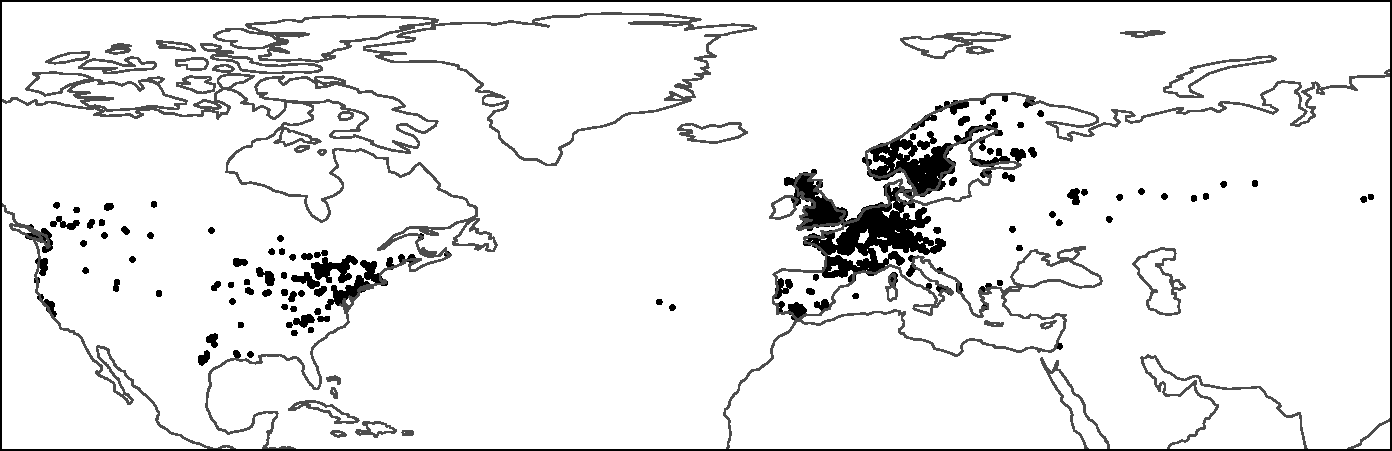
\includegraphics[width=0.9\textwidth]{Figures/Ps_presence_map.pdf}
    \caption{\textbf{Training presence records for modeling the
            distribution of \textit{Philaenus spumarius.}}}
    \label{fig:Ps_presence_map}
\end{figure}

In addition, we randomly generated pseudo-absences, also known as
background points, using ``The Three-Step'' method proposed in
\cite{iturbide_framework_2015}. This method incorporates a model performance
criterion to determine the optimal sampling background extent, thereby ensuring
that the model fitting was not adversely affected by the pseudo-absence
sampling. Nevertheless, we accounted for the potential variability introduced
by randomly selecting points from the background by performing 10 realizations
of this sampling process. A total of 4956 pseudo-absences (three times the
number of presences) were used in each realization.

Model evaluation was performed using a $k$-fold cross-validation approach
(where $k = 10$) and the resulting AUCs (Area Under the ROC Curve) consistently
exceeded $0.9$ within the range of $0$ to $1$, with a value of $1$ indicating
perfect prediction and $0.5$ indicating no discriminatory power (i.e. random
guessing). Finally, the calibrated models were used to predict the suitability
of \textit{P. spumarius} in the reference historical period (2003-2022) and
under increasing global warming scenarios (panels b, d, f, h in
\cref{fig:Xf_Ps_suitability_change}).

\subsection{Risk velocity}

To assess the dynamic nature of the risk index and its spatial propagation,
we introduced the concept of risk velocity, a metric analogous to the recently
proposed concept of climatic velocity \cite{Loarie2009}. The risk velocity
represents the rate at which the risk index changes over time and spreads
across different locations. From an epidemiological perspective, risk velocity
can be thought as the speed and direction the host would need to move to
maintain its current risk conditions under climate change. Risk velocities were
defined following the definition of climate velocity, as the ratio of the risk
temporal trend and the risk spatial gradient in each cell. Thus, the units for
the risk velocity correspond to kilometres per year ($km/\mathrm{year}$). Risk
velocities were computed using the VoCC R package \cite{VoCC, VoCC_paper}.

\subsection{Maps}

The maps of all Figures in the paper (\cref{fig:Ps_presence_map} to
\cref{fig:vineyards}) and in the Supplementary Information file were made with
Python 3.11 \cite{Python} using the package Cartopy v0.21.1 \cite{Cartopy,
    Cartopy_zenodo}.

\section{Results}

\subsection{Present and future climate suitability for \textit{Xylella
        fastidiosa} (PD) and \textit{Philaenus spumarius}}

To gain a deeper understanding of how climate change affects each component
of the pathosystem, we performed a separate analysis of climatic suitability
conditions for \xf{} and \textit{P. spumarius}. The thermal dependence of \xf{}
growth and survival within the infected vine was mechanistically modeled by
probability functions relating the accumulation of modified degree days
($MGDD$) and cold degree days ($CDD$) to symptom development and recovery,
$\mathcal{F}(MGDD)$ and $\mathcal{G}(CDD)$, respectively (see Methods).
Climatic suitability for pathogen establishment was then determined by
$\mathcal{F}(MGDD)\cdot\mathcal{G}(CDD)$, i.e. the overall probability of
symptom development during the growing season and subsequent survival for
overwintering infection (see Methods).	For \textit{P. spumarius}, climatic
suitability was modeled using an SDM based on a previous study
\cite{Godefroid2022_vector}, with the climatic moisture index
\cite{willmott_more_1992} and spring maximum temperatures  as key predictors
(see Methods). Both analyses were evaluated under current (2003-2022) and
future climate conditions considering scenarios of increasing global warming
(+1.5ºC, +2ºC, +3ºC, and +4ºC) based on the latest generation of regional
climate projections covering Europe \cite{jacob_regional_2020} (see Methods).

Progressive global warming increases the accumulation of MGDD during the
growing season and reduces the recovery rate (i.e. CDD) during winter, thus
favouring the geographic expansion of the pathogen
(\cref{fig:Xf_Ps_suitability_change} and \cref{fig:Xf_Ps_suitability}).
Conversely, increasing temperatures tend to reduce the climatic suitability of
vectors in more arid areas of southern Europe leading to a progressive
migration to higher areas and latitudes in continental regions in search of
climatic refuge. These general trends hold for both organisms under the +2, +3
and +4 ºC temperature increase scenarios
(\cref{fig:Xf_Ps_suitability_change}).

The mechanistic approach to modelling pathogen establishment risk enables
each of the two opposing directional processes of growth and survival (MGDD vs.
CDD) to be appropriately weighted in the final result. For example, the
Bordeaux region in western France has not been at risk due to low cumulative
MGDD and low winter protection effect.	In the transition from the +1.5ºC
scenario to the +4ºC scenario, this area will experience a spectacular increase
in risk mainly due to the expected summer warming
(\cref{fig:Xf_suitability_explainability}). Conversely, areas of Central
Europe such as Hungary and Serbia already experience suitable conditions for
pathogen growth in a +1.5ºC scenario ($\mathcal{F}(MGDD) > 0.6$); however, cold
winters tend to eliminate any potential summer infection $[\mathcal{G}(CDD) <
            0.3]$ (\cref{fig:Xf_suitability_explainability}). Climate change
would further
increase the growth of the pathogen  and reduce the winter curing effect in
Central Europe, ultimately exposing the region to \xf{}
(\cref{fig:Xf_suitability_explainability}).

\begin{figure}[H]
    \centering

    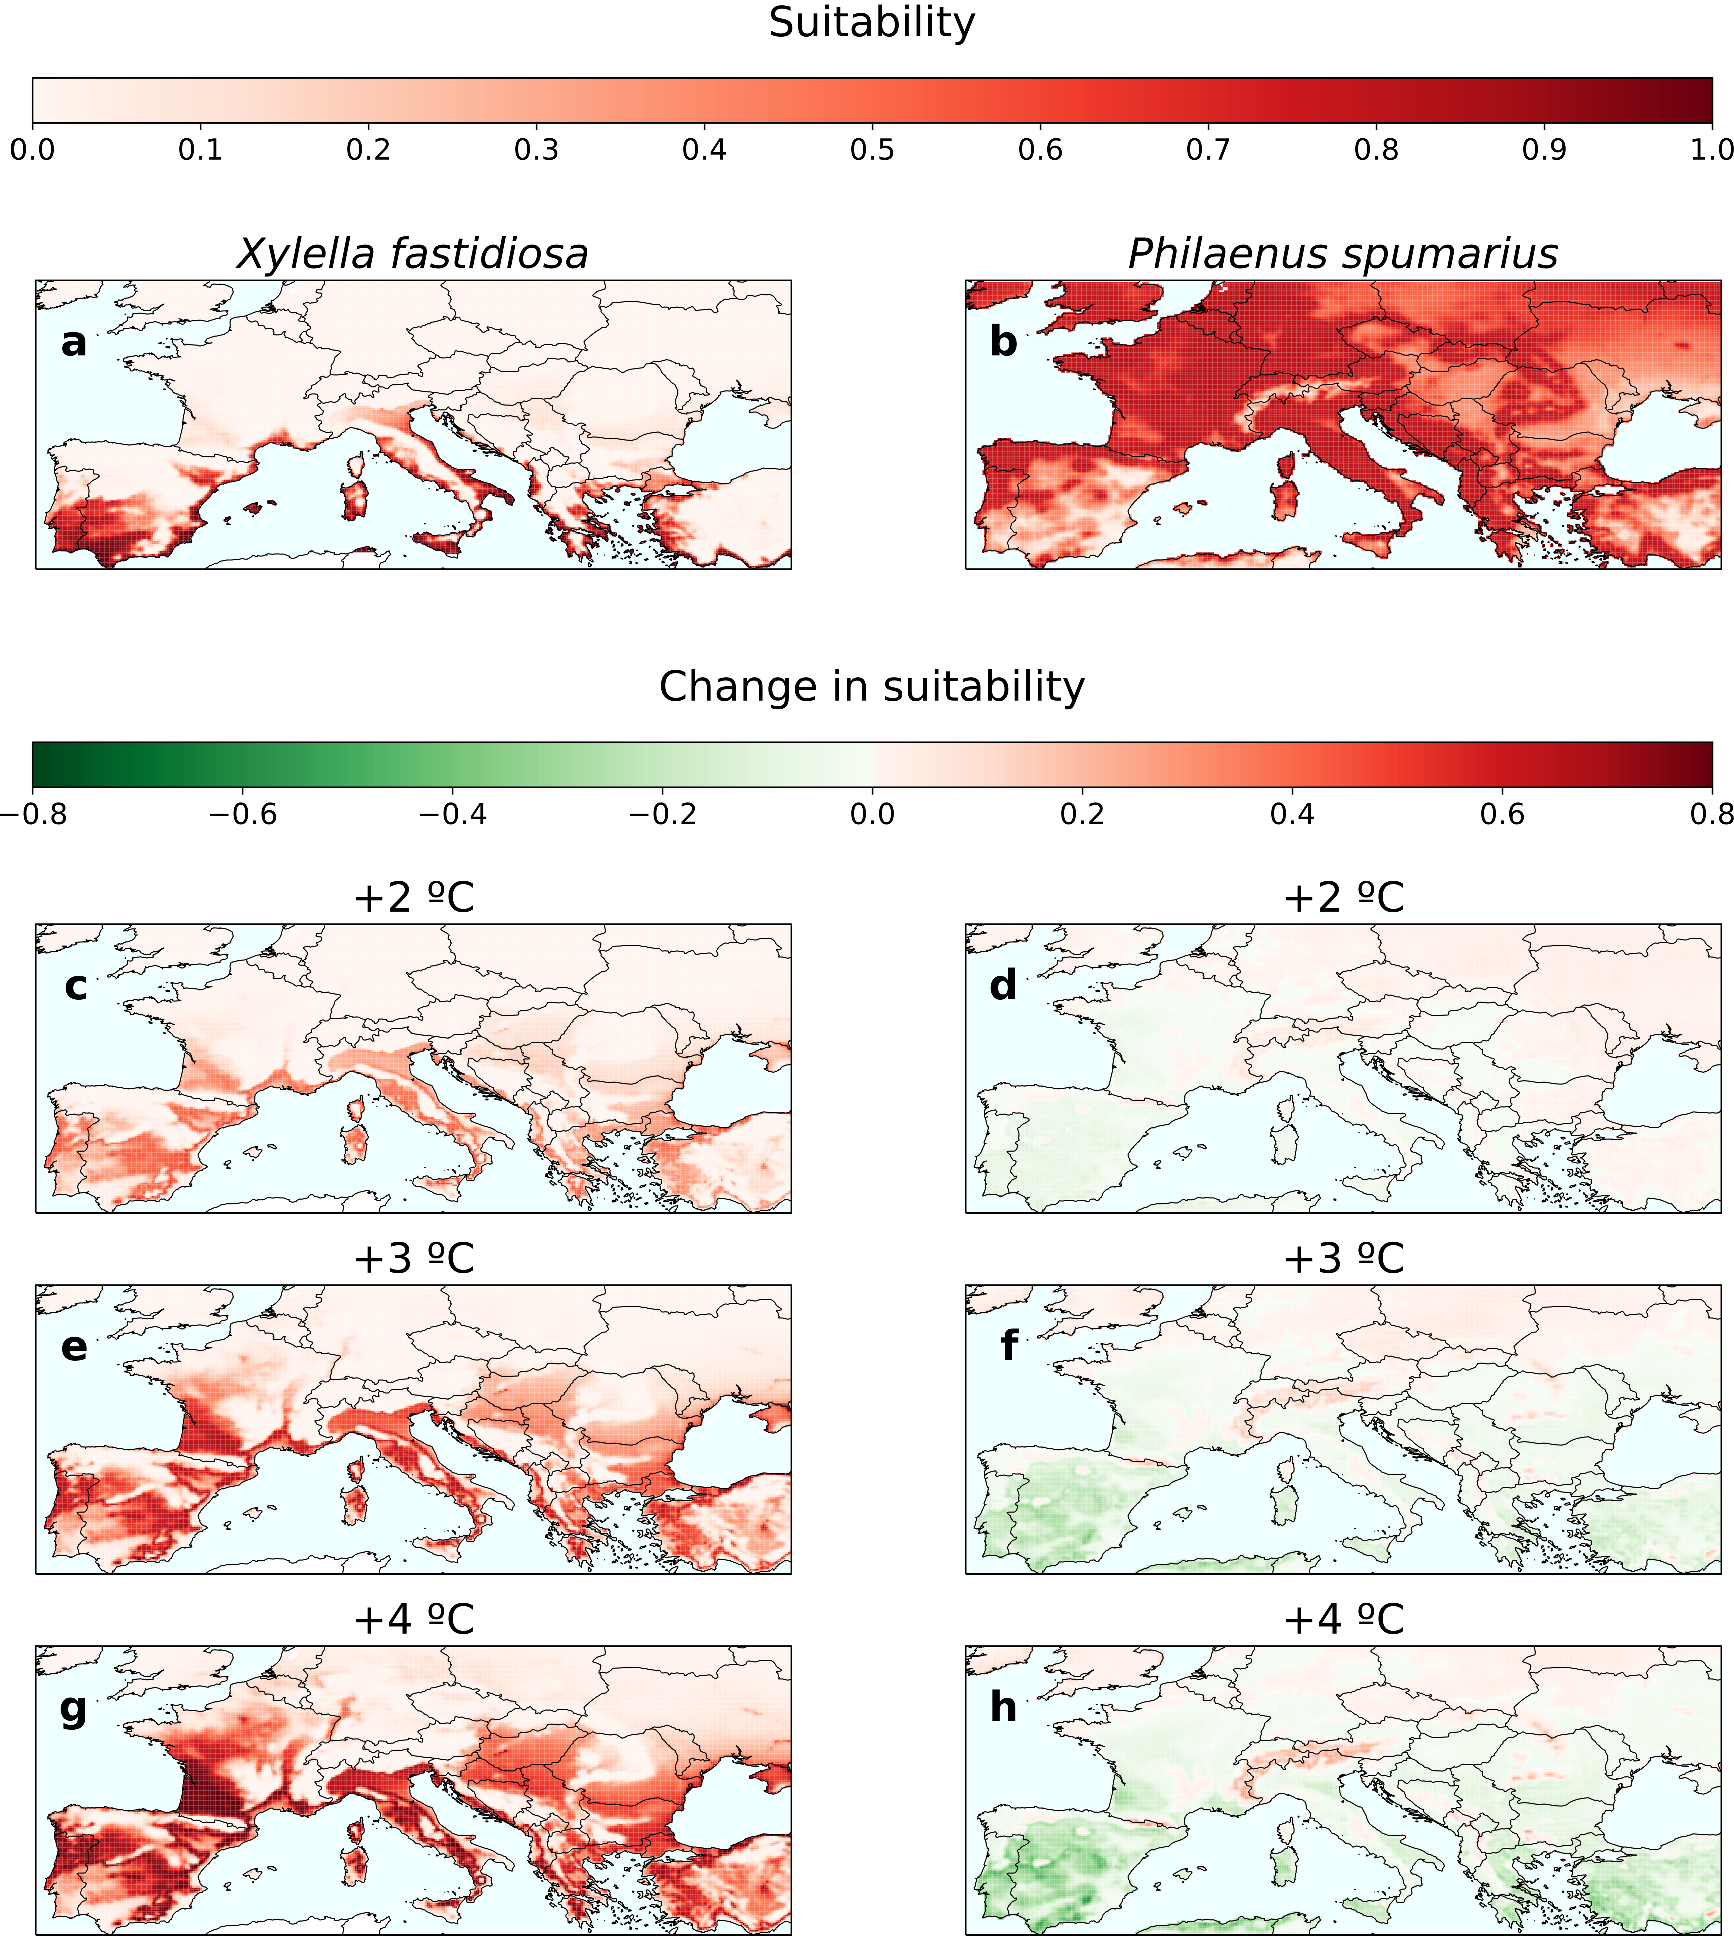
\includegraphics[width=\textwidth]{Figures/Xf_Ps_suitability_differences.pdf}
    \caption{\textbf{Changes in \xf{} and \textit{P. spumarius} climatic
            suitability (i.e. probability of occurrence) under different
            climate
            projections compared to the current scenario (2003-2022).} Current
        climatic
        suitability for the pathogen (a) and the vector (b). In an increasing
        temperature scenario (+2ºC , +3ºC and +4ºC) the climatic suitability
        for the
        pathogen geographically expands in southern Europe and moves northwards
        (c, e
        and g) while the climatic suitability for the vector decreases (d, f
        and h).
        The suitability values for each scenario correspond to a 20-year
        average.}
    \label{fig:Xf_Ps_suitability_change}
\end{figure}

\subsection{Pierce's disease risk projections under climate change}

The limited intersection between the climatic suitability ranges for the
pathogen and the vector (\cref{fig:Xf_Ps_suitability_change}a and b) suggests
a marginal  risk of PD epidemics in Europe. Since disease transmission requires
a vector, the climate-suitability maps for \textit{P. spumarius}  indicate a
lower risk and potential economic impact of \textit{X. fastidiosa}-induced
diseases on any host in southern Europe, particularly Spain, than previously
predicted \cite{Schneider2020}. Realistic risk maps require a defined
epidemiological framework to account for inter-annual climate variation and
transmission in disease dynamics, in addition to accounting for changes in the
distribution of climatic conditions favorable to the pathogen and vector (i.e.
climatic suitability). Our epidemic risk model focuses on delimiting the
disease dynamics by simulating an epidemic process in which the emergence of
newly exposed hosts is influenced by the climatic suitability of the vector,
while the transition to the infectious state is driven by the climatic
suitability for \xf{} chronic infections. The effective growth rate of the
infected host population over the simulated period is used to derive a risk
index $r$, bounded between $-1$ and $1$. Within this modeling framework,
different risk categories naturally emerge: no
risk ($r<-0.1$), transition zone ($-0.1\leq r<0.1$), low risk ($0.1\leq
    r<0.33$), moderate risk ($0.33\leq r<0.66$) and high risk ($r\geq0.66$).
For further details see the Methods section and the original paper
\cite{GimenezRomero2022_CommsBio}.

\begin{figure}[H]
    \centering
    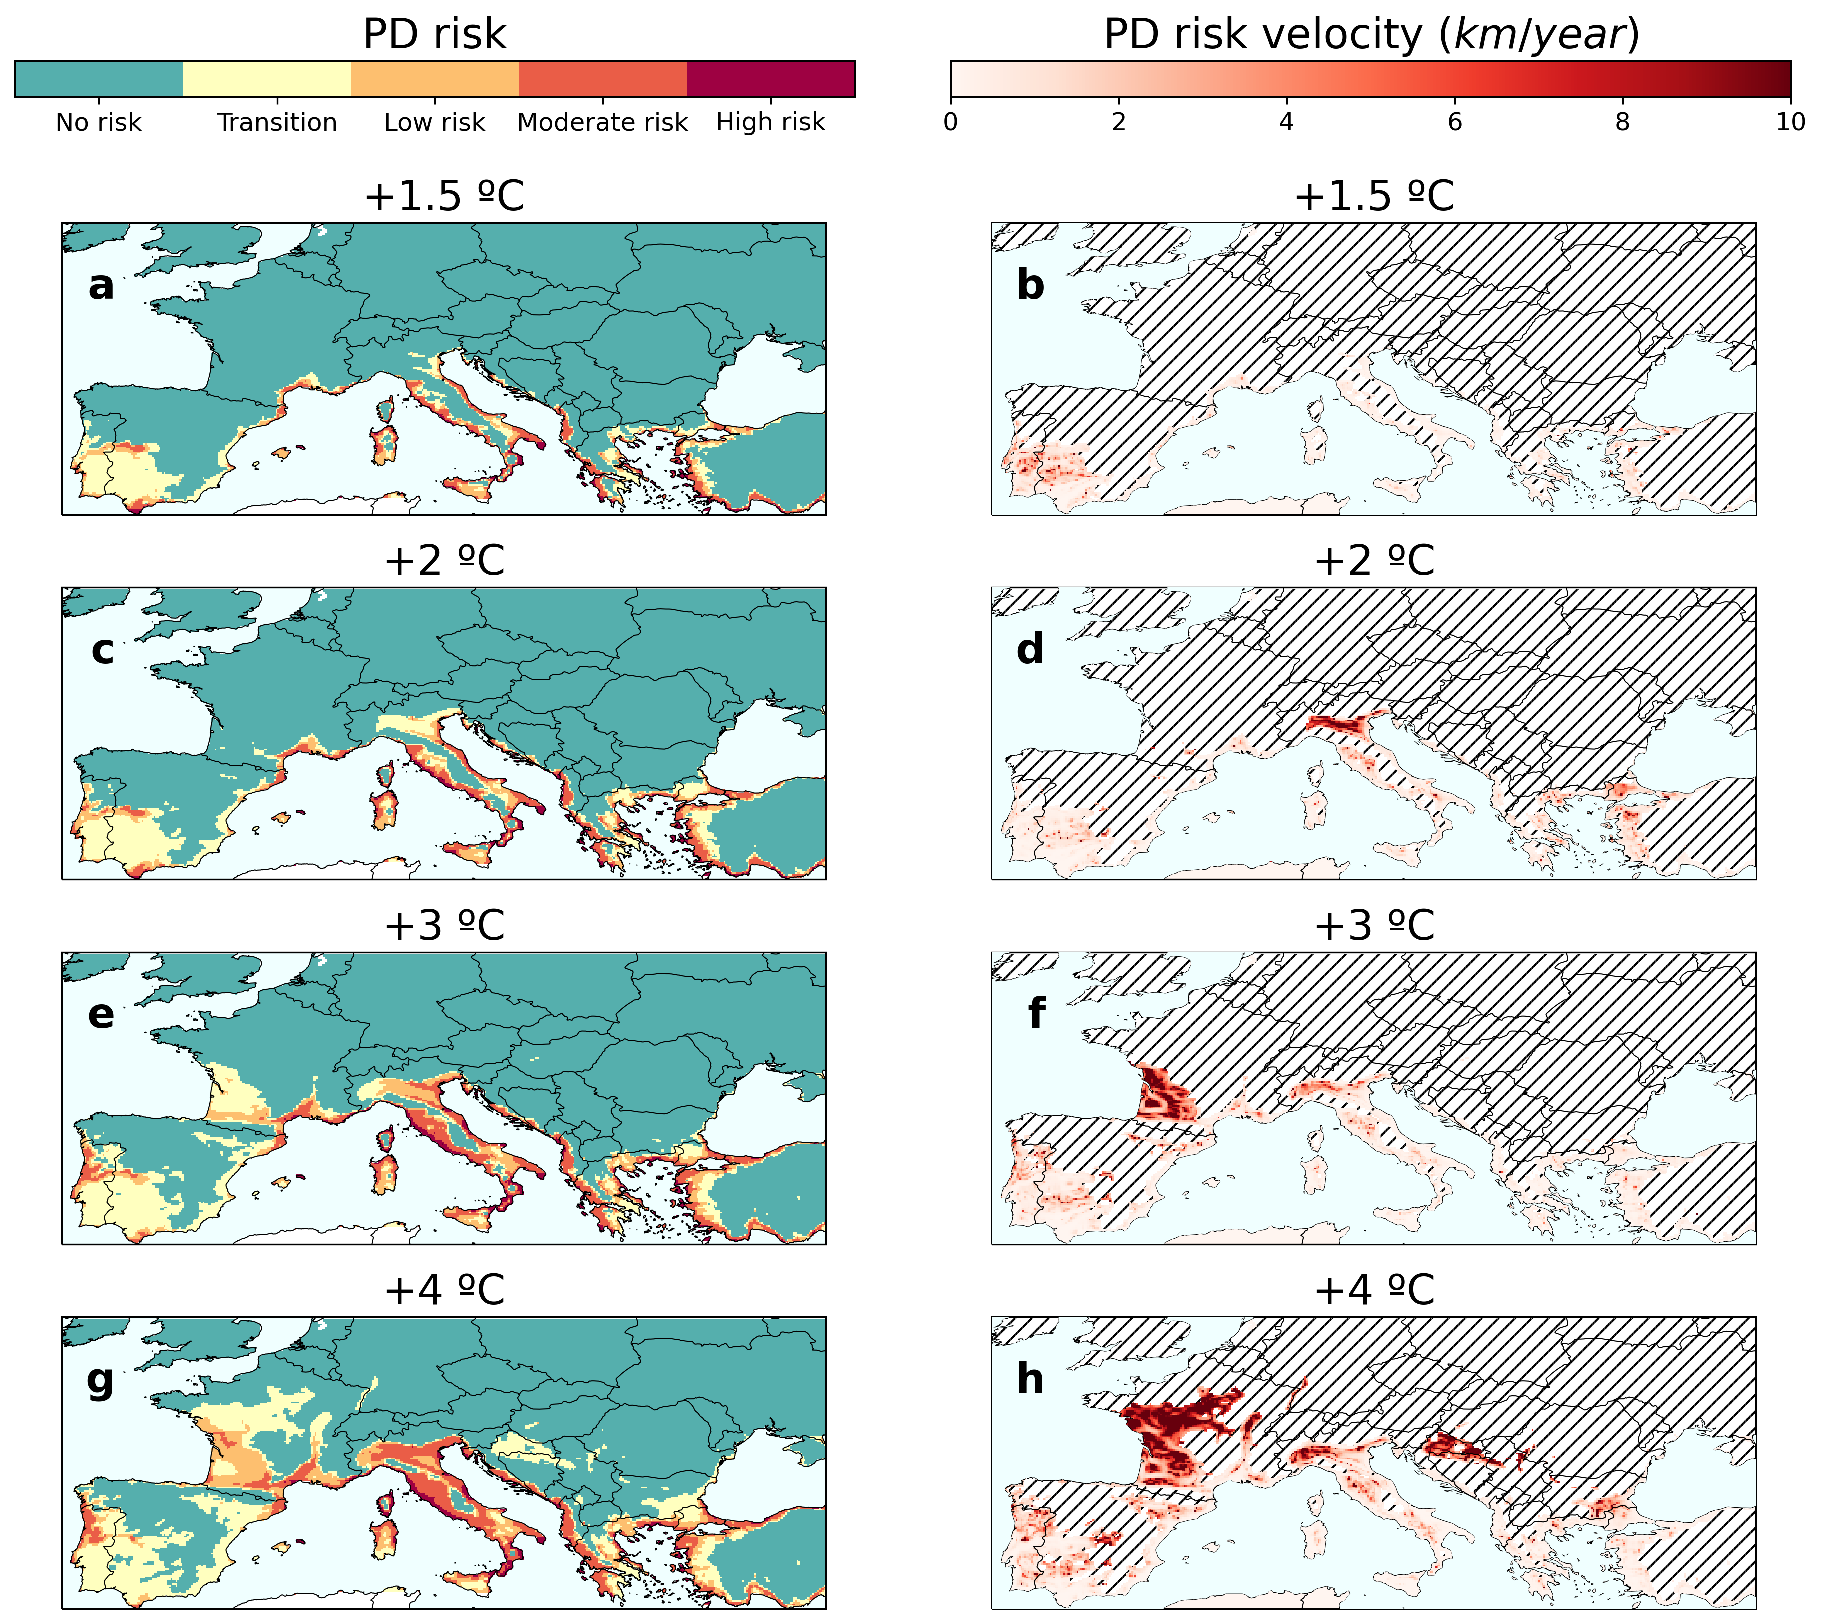
\includegraphics[width=1\textwidth]{Figures/Future_risk_PD.pdf}
    \caption{\textbf{PD risk maps and associated risk velocities under
            different climate projections.} (a,b) +1.5ºC climate projection.
        (c,d) +2ºC
        climate projection. (e,f) +3ºC climate projection. (g,h) +4ºC climate
        projection. Risk velocities have been calculated only in  risk zones,
        $r > 0$,
        in each scenario. Hatched lines in panels (b,d,f,h) indicate no risk
        zones
        where risk velocities have not been calculated.}
    \label{fig:PD_future_risk_zones}
\end{figure}

Global warming (+1.5ºC, +2ºC, +3ºC, and +4ºC) is expected to increase the
risk of PD epidemics in southern Europe, with France, Italy and Portugal being
particularly affected (\cref{fig:PD_future_risk_zones} and
\cref{fig:PD_future_risk}). This general trend affects each of the risk
categories under the different climate change scenarios
(\cref{fig:PD_future_risk_velocity}). Furthermore, we observed that a global
temperature increase above +3ºC represents a tipping point for the possible
spread of PD beyond the Mediterranean (\cref{fig:PD_future_risk_zones} and
\cref{fig:PD_future_risk}). To quantify the potential spread of PD, we
calculated risk velocity, an index that allows us to identify areas where risk
is changing  or spreading rapidly (see Methods). We found a consistent and
notable increase in the mean risk velocity within most of the identified risk
zones (\cref{fig:PD_future_risk_zones} and \cref{fig:PD_future_risk_velocity}),
increasing from almost 1 km y$^{-1}$ to 5
km y$^{-1}$ as the temperature rises from a +1.5ºC to a +4ºC scenario
(\cref{tab:risk_vel}). This acceleration is evident when we
compare that in
the +1.5ºC scenario, approximately 6\% of the grid cells have risk velocities
greater than 5 km y$^{\mathrm{-1}}$, while this value increases to 50\% in the
+4ºC scenario (\cref{tab:risk_vel}). Furthermore, our estimates of
PD risk
velocity are broadly consistent with estimates of the velocity of temperature
change \cite{Loarie2009}, indicating that shifts in PD risk in our model
adequately track climate change.

\begin{figure}[H]
    \centering
    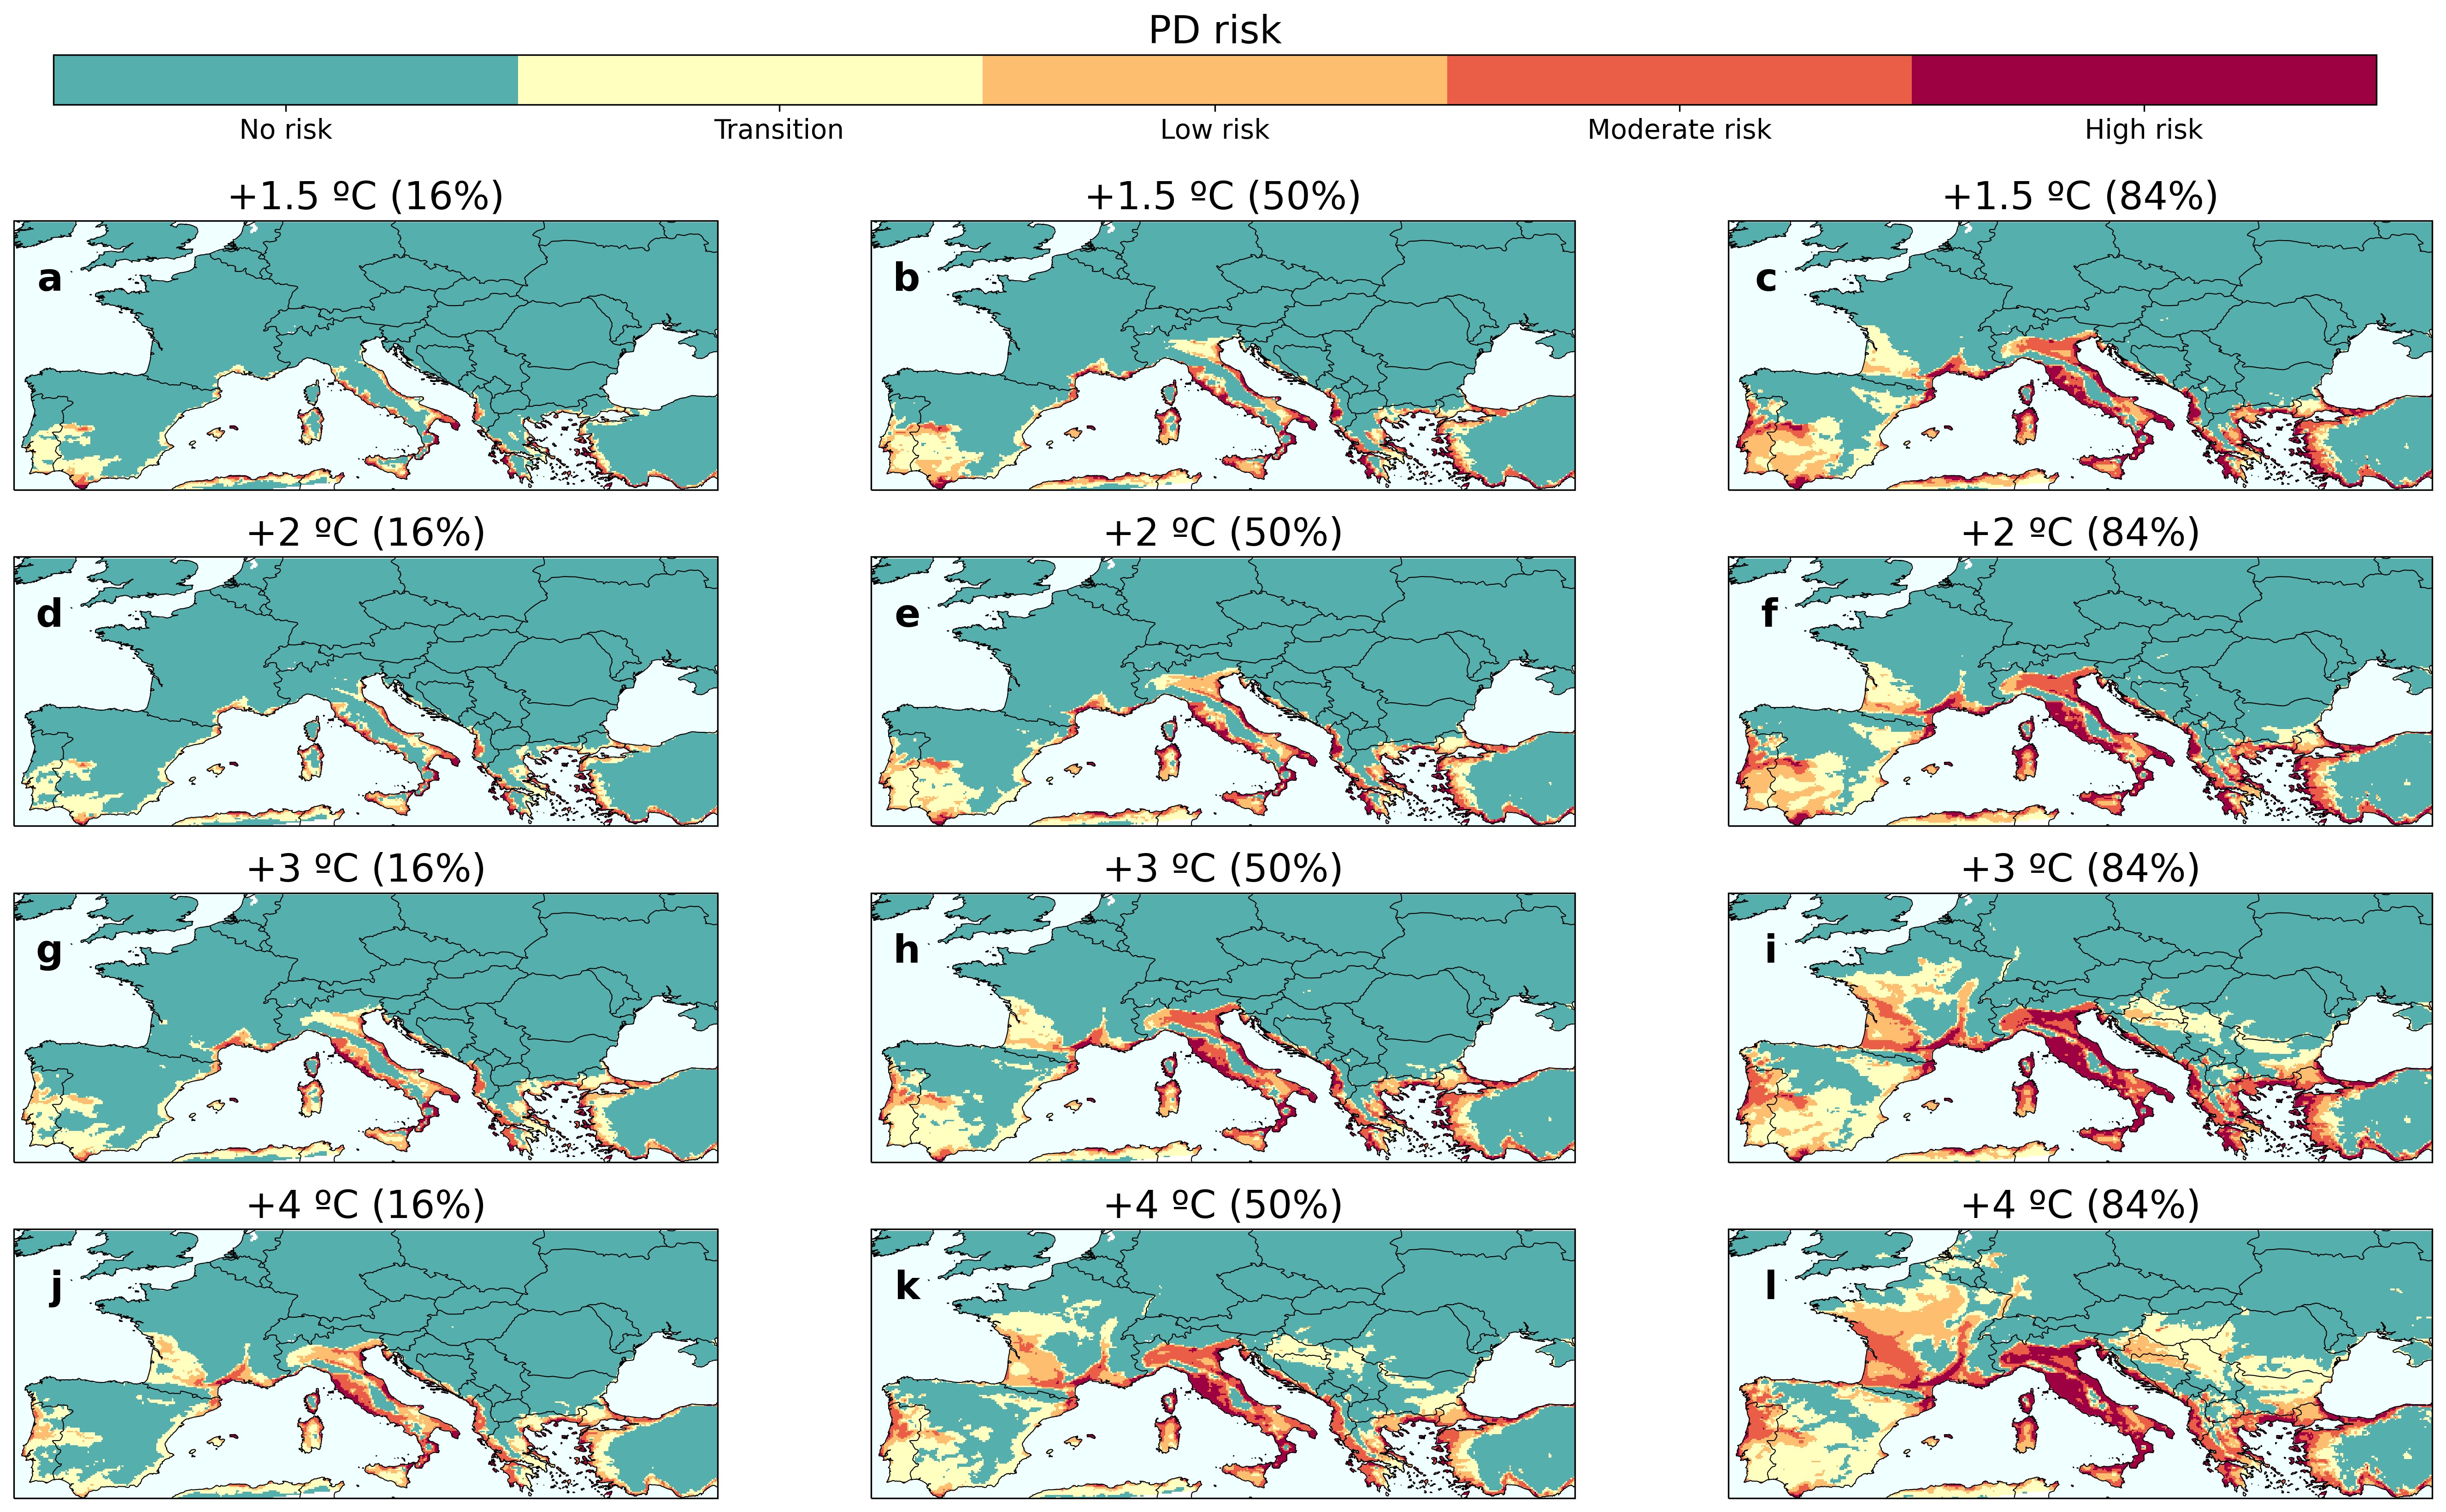
\includegraphics[width=\textwidth]{Figures/Uncertainty.png}
    \caption{\textbf{Uncertainty in PD risk projections for climate change
            warming levels}. The maps show the result of the median risk values
        of the set
        of 40 regional climate model projections for each level of temperature
        increase
        (b, e, h, k) and the uncertainty of the projections considering the $1
            \sigma$
        deviations from the median, this is, the 16\% (a, d, g, j) and 84\% (c,
        f, i,
        l) percentiles. For each warming level (each row), the projected risk
        of PD is
        comprised between the results shown in the 16\% percentile (first
        column) and
        those shown in the 84\% percentile (last column) with 68\% probability
        (1$\sigma$).}
    \label{fig:uncertainty}
\end{figure}

\cref{fig:uncertainty} shows the uncertainty in the projections of the PD
risk map, comparing the 16th and 84th percentiles ($1\sigma$) from the set of
40 regional climate models to the median risk map. The spatial distribution of
PD risk is robust across models, while the uncertainty in the level of warming
is bounded by a $\pm$ 1ºC increase (\cref{fig:uncertainty}), e.g. the median
spatial distribution of risk obtained for a +3ºC warming level is expected to
occur between the +2ºC and the +4ºC scenarios under a 1$\sigma$ confidence
level. This means that, depending on the specific model, a given spatial
distribution of risk (e.g., \cref{fig:uncertainty} h) may manifest under a +4°C
warming scenario in more conservative projections or a +2°C warming scenario in
others, while most models project it for a +3°C warming level. This indicates a
high degree of confidence in the location and projected severity of future
outbreaks, but greater uncertainty in their timing.

In order to improve the accuracy of the risk maps and the  relative impact
of PD, we carried out a comprehensive analysis at multiple scales, from the
national level to the regions with Protected Designation of Origin (PDO) and
finally taking into account the distribution of vineyards. This approach allows
us to disaggregate the results at different administrative levels to facilitate
the design of risk management and the implementation of appropriate
phytosanitary measures.

\begin{figure}[H]
    \centering

    \includegraphics[width=\textwidth]{Figures/Future_risk_country_and_vineyards.pdf}
    \caption{\textbf{Multi-scale spatial analysis of PD future risk in
            Europe.} (a, c, e, g) Percentage of country areas at risk ($r>0.1$)
        for each
        climate projection. (b, d, f, h) PD risk zones in Protected Designation
        of
        Origin (PDO) wine regions for each climate projection. PDO data was
        obtained
        from \cite{Candiago2022}. The corresponding interactive analysis at the
        vineyard level can be found in \cite{Webpage}}
    \label{fig:vineyards}
\end{figure}

Overall, our model simulations show a consistent
increasing trend in the risk of PD in Europe under all climate change
scenarios. The percentage of land area at risk in Europe increases from 0.32\%
in the +1.5ºC scenario to 1.87\% in the +4ºC, while the number of regions with
PDO at risk increases from 18.17\% to 47.32\% . The vineyard area  increases
from 18.67\% to 40.35\% (\cref{tab:general}). At country level
Portugal and
Greece face the highest overall risk, escalating from 12\% and 2\% of their
area  in the +1.5ºC scenario to a striking 47\% and 63\%  respectively in a
+4ºC scenario. In contrast, countries such as France and Italy experience a
smaller but still significant increase in risk area, never exceeding the 20\%
threshold, while Spain, the third largest wine producer, shows a decreasing
trend in risk areas above the +2ºC scenario (\cref{fig:vineyards} and
\cref{tab:countries}). Such contrasting patterns in PD risk between
countries
only emerge when using our modelling framework.

A different picture emerges when looking at the spatial distribution of PDO
regions and vineyards. For example, PD risk within French and Italian PDO
regions increases significantly from 13.4\% and 45.8\% in a +1.5ºC scenario to
41.6\% and 82.7\% in a +4ºC scenario (\cref{fig:vineyards} and
\cref{tab:countries}), while the percentage of vineyard area at
risk rises
from 24.21\% and 57.49\% in a +1.5ºC scenario to an astonishing 80\% in a +4ºC
scenario. Important European PDOs would be at risk from a warming of  +2ºC,
such as parts of the southern Rhône Valley (Châteneuf du Pape), Provence and
Languedoc in France, Penedés in Spain, Bairrada in Portugal, and Chianti and
Brunello di Montalcino among others in Italy (see Supplementary Information). A
detailed interactive analysis of the impact of PD in European PDO regions and
vineyards is available on our website \cite{Webpage}.

\section{Discussion}

Previous research has attempted to assess the potential geographic
distribution of  \xf{} subspecies, the insect vector \textit{P. spumarius} and
PD using species distribution models (SDMs) under future climates. While these
climate-suitability-based predictions provide insights into the ecological
niche of key disease players, bioclimatic correlative models neglect disease
dynamics, a key factor in avoiding disease overestimation
\cite{GimenezRomero2022_CommsBio}. Unlike previous attempts, our approach
integrates
the compound effect of climate change in the pathosystem using a mechanistic
epidemiological model to overcome these limitations.  Unlike dimensionless
climatic suitability indexes or disease probabilities used in SDMs, the risk
index, $r$, in our model provides information on the expected growth rate in
the event of an outbreak . Furthermore, the risk index is not fixed but varies
annually depending on the weather conditions of the previous years.
Inter-annual climate variability thus has an impact on disease dynamics,
especially in areas where the risk index is lower.  Another feature of our risk
predictions is their lack of ambiguity, which should not be confused with
certainty. Risk estimates are based on $R_0$, which depends on the insect
vector population \cite{GimenezRomero2022_PRE}, among other factors. Areas
where
$r<-0.1$ permanently cannot theoretically support an outbreak, and the
population of infected plants will decline over time. For example, our model
clearly indicates that there is no risk of PD in the UK. This is not an
arbitrary threshold; it  is given by the epidemiological model.  It is
therefore very likely that the absence of PD in continental Europe is a
consequence of low risk indices and that it has only become established in
certain coastal areas since the late 1990s. On the contrary, the risk index in
the Mediterranean islands has remained moderately high with little variation
over the last 40 years \cite{GimenezRomero2022_CommsBio}.

Because Pierce's disease has only affected vineyards on the island of
Mallorca \cite{moralejo2019insights}, little attention has been paid to the
risk of it reaching continental vineyards. Our risk model indicates why this
possibility was very low until the mid-90s, and what the conditions were for it
to occur on the Mediterranean islands \cite{GimenezRomero2022_CommsBio}.  In
this work,
we clearly show that  with increasing temperatures PD will become a serious
threat to important wine-growing areas in southern Europe that were not
previously at risk. A key finding of our study is the identification of a
tipping point for the risk of PD establishment at a global mean temperature
increase of +3ºC. Beyond this threshold, the risk of PD spreading north of the
Mediterranean region becomes remarkably higher, while the risk of PD epidemics
in Portugal, Italy and France (\cref{fig:PD_future_risk_zones}) undergoes a
significant quantitative leap. This suggests that as global temperatures
continue to rise, the range of PD may expand into new territories. Indeed, the
projected increase in risk velocities under higher warming scenarios further
emphasizes the potential for rapid spread of PD into previously unaffected
regions (\cref{fig:PD_future_risk_zones}).

Pest risk map projections are subject to uncertainties inherent in the
variability of climate model predictions \cite{venette2010pest}. While previous
studies on pathogen and vector distributions have been based on a limited
number of climate models, our risk maps are based on the most modern set of
regional climate projections produced by the EURO-CORDEX initiative, reflecting
the state-of-the-art knowledge (\cref{tab:GCM-RCM}). This allows us to
adequately estimate the uncertainty of the resulting PD risk map projections
for each temperature rise scenario. This confirms that although the spatial
distribution of the risk of establishment is robust, there is an uncertainty of
$\pm$ 1ºC in the level of warming (\cref{fig:uncertainty}). The models are
therefore fairly good at  pointing  where the increased risk will occur, but it
is more difficult to know when it will be reached.

Overall, our results highlight the contrasting effect of climate change on
PD risk distribution in Europe, revealing it as a multi-factor and multi-scale
process (\cref{tab:countries}). Climate change has an opposite effect on each
component of the pathosystem, enhancing areas of potential chronic PD
infections while diminishing the suitable geographic range for the vector. At
the same time, the characteristic spatial scale at which risk is assessed
strongly influences conclusions. At the country level, there are significant
variations in the extent of accumulated risk between different projections.
However, when analyzed at a finer scale, such as at the level of PDO regions or
vineyards, the results change completely. Countries that previously had
marginal areas at risk now show a higher percentage of PDO regions and vineyard
at risk. These results underlie the urgency of tailored mitigation and
adaptation strategies to protect vineyards and PDOs, considering their specific
spatial distribution and risk index, as well as the potential impacts of
climate change.

Our results are influenced by the intrinsic uncertainty associated with the
correlative models used to determine the spatial distribution of the vector,
the epidemiological parameters, and the uncertainties in the climatic
projections. Although the spatial resolution of our climate projections is
considered to be high, it may not capture the complex micro-climate structure
found in certain European wine-producing regions. Therefore, risk assessment
results could differ locally with higher-resolution data. In addition, we have
not considered the possible influence of climate change on latitudinal and
altitudinal shifts in the distribution of European vineyards
\cite{hannah2013climate,moriondo2013projected}, as this would only affect the
calculation of the percentage of vineyard surface at risk but not the actual
spatial distribution of risk. In any case, the risk estimates for the PDO
regions include areas much larger than the areas of planted vines, which allows
some margin in the adaptation and migration of the vineyards to different
micro-climatic conditions. In addition, the PDO and vineyard databases used in
this study are also have their own limitations. Future studies incorporating
more refined modeling techniques, specific regional grapevine varieties, crop
management and improved data resolution would enable a more nuanced
understanding of PD risk and its potential impact at the local scale.

It is noteworthy that the mathematical framework employed in this study
could be applied to other \textit{Xylella fastidiosa} diseases, such as Almond
Leaf Scorch Disease or Olive Quick Decline Syndrome and, more generally, to
other vector-borne plant diseases. However, this requires the availability of
some specific data and conducting some experiments. First, data for the
temperature-dependent growth rate of the pathogen is needed to build the
function that computes the MGDD. Then, symptom development experiments need to
be carried out to build the $\mathcal{F}(MGDD)$ and $\mathcal{G}(CDD)$
functions that relate symptom development with temperature. Finally, the
spatial distribution of the agent responsible for disease transmission is
desired. Of course, using presence/absence data one can use SDM to obtain this
spatial distribution.

Climate change is currently one of the biggest challenges for EU
agricultural policy \cite{fellmann2018major}. Quantitative regional predictions
of climate change on emerging diseases, such as this one, provide a valuable
and unambiguous tool for decision-making. In our approach to the problem, risk
indexes not only include information on where or where not PD may become
established, but also reflect the exponential growth rate of potential
epidemics, which are directly related to their potential economic impact. In
addition, risk indices and velocities provide a dynamic framework for assessing
the feasibility of eradication efforts when \xf{} is detected in a new area,
providing critical information for strategic crop protection. Our study
evidences the need to selectively allocate more resources to surveillance and
research on PD in southern European countries, considering the associated
uncertainties. This strategic allocation of resources based on risk assessment
can help to prioritise proactive measures and effectively manage the potential
impact of PD in different European countries.

Our research highlights the complex dynamics of PD and its relationship
with climate change. By adopting an interdisciplinary approach that integrates
climate projections, epidemiological modelling, and spatial analysis, we
provide valuable insights into the potential establishment and spread of PD in
European wine-growing regions from the country to the vineyard levels. Our
study demonstrates that an accurate assessment of the risk of PD establishment
requires a nuanced understanding of the vector-plant-pathogen-climate system
and the explicit consideration of the vineyard spatial setting. These findings
can inform decision-making processes and support the development of effective
strategies to mitigate the risks posed by PD and safeguard the future of
viticulture in the face of a changing climate.